%%%%%%%%%%%%%%%%%%%%%%%%%%%%%%%%%%%%%%%%%
% Journal Article
% LaTeX Template
% Version 1.0 (25/8/12)
%
% This template has been downloaded from:
% http://www.LaTeXTemplates.com
%
% Original author:
% Frits Wenneker (http://www.howtotex.com)
%
% License:
% CC BY-NC-SA 3.0 (http://creativecommons.org/licenses/by-nc-sa/3.0/)
%
%%%%%%%%%%%%%%%%%%%%%%%%%%%%%%%%%%%%%%%%%

%----------------------------------------------------------------------------------------
%	PACKAGES AND OTHER DOCUMENT CONFIGURATIONS
%----------------------------------------------------------------------------------------

\documentclass[twoside]{article}

\usepackage{lipsum} % Package to generate dummy text throughout this template
\usepackage{url}
\usepackage{hyperref}
\usepackage[sc]{mathpazo} % Use the Palatino font
\usepackage[T1]{fontenc} % Use 8-bit encoding that has 256 glyphs
\linespread{1.05} % Line spacing - Palatino needs more space between lines
\usepackage{microtype} % Slightly tweak font spacing for aesthetics
\usepackage{graphicx}
\usepackage[hmarginratio=1:1,top=32mm,columnsep=20pt]{geometry} % Document margins
\usepackage{multicol} % Used for the two-column layout of the document
\usepackage{hyperref} % For hyperlinks in the PDF

\usepackage[hang, small,labelfont=bf,up,textfont=it,up]{caption} % Custom captions under/above floats in tables or figures
\usepackage{booktabs} % Horizontal rules in tables
\usepackage{float} % Required for tables and figures in the multi-column environment - they need to be placed in specific locations with the [H] (e.g. \begin{table}[H])

\usepackage{lettrine} % The lettrine is the first enlarged letter at the beginning of the text
\usepackage{paralist} % Used for the compactitem environment which makes bullet points with less space between them

\usepackage{abstract} % Allows abstract customization
\renewcommand{\abstractnamefont}{\normalfont\bfseries} % Set the "Abstract" text to bold
\renewcommand{\abstracttextfont}{\normalfont\small\itshape} % Set the abstract itself to small italic text


\usepackage{titlesec} % Allows customization of titles
%\titleformat{\section}[block]{\large\scshape\centering{\Roman{section}.}}{}{1em}{} % Change the look of the section titles 
\usepackage{fancyvrb}
\usepackage{fancyhdr} % Headers and footers
\pagestyle{fancy} % All pages have headers and footers
\fancyhead{} % Blank out the default header
\fancyfoot{} % Blank out the default footer
\fancyhead[C]{CS497 - Haskell In The Cloud $\bullet$ November 2012} % Custom header text
\fancyfoot[RO,LE]{\thepage} % Custom footer text

\usepackage{listings}
\lstloadlanguages{Haskell}
\lstnewenvironment{code}
    {\lstset{}%
      \csname lst@SetFirstLabel\endcsname}
    {\csname lst@SaveFirstLabel\endcsname}
    \lstset{
      basicstyle=\footnotesize,
      %flexiblecolumns=true,
      frame=single,
      basewidth={0.5em,0.45em},
     }

%----------------------------------------------------------------------------------------
%	TITLE SECTION
%----------------------------------------------------------------------------------------

\title{\vspace{-15mm}\fontsize{24pt}{10pt}\selectfont\textbf{CS497 - Haskell
    In The Cloud}} % Article title

\author{
\large
\textsc{Pankaj More}\\[2mm] % Your name
\normalsize Indian Institute of Technology, Kanpur \\ % Your institution
\normalsize \href{mailto:pankajm@iitk.ac.in}{pankajm@iitk.ac.in} % Your email address
\vspace{-5mm}
}
\date{}
\setcounter{tocdepth}{4}
%----------------------------------------------------------------------------------------

\begin{document}

\maketitle % Insert title

\thispagestyle{fancy} % All pages have headers and footers

%----------------------------------------------------------------------------------------
%	ABSTRACT
%----------------------------------------------------------------------------------------

\begin{abstract}

  With the increasing need for large scale data centers for industrial
  and research purposes, the difficulty of distributed programming is
  becoming more apparent. Some languages are bettter suited for large
  scale distributed programming. Erlang , with its actor model,
  particularly has proven quite successful for programming large
  clusters. There have been recent advances in Haskell in area of
  distributed programming. Cloud Haskell, a recent implementation, is
  a library in haskell for developing programs for a distributed
  computing environment. It provides a message passing model for
  communication between programs, inspired by Erlang. Apache Pig is a
  platform for writing scripts in high-level language for converting
  into hadoop map-reduce jobs. In this project , we have looked into
  the specific advantages Cloud Haskell brings to programmers for
  distributed programming and look at how a Pig-like DSL on top of
  CloudHaskell could be implemented.

\end{abstract}

%----------------------------------------------------------------------------------------
%	ARTICLE CONTENTS
%----------------------------------------------------------------------------------------
\tableofcontents 
%\begin{multicols}{2} % Two-column layout throughout the main article text

\pagebreak

\section{Introduction}

\lettrine[nindent=0em,lines=3]{T} oday with increasing usage of large
data centers \cite{newagedcs} by enterprises, the abilty to program on
huge datasets has become more important than ever. When programs
executing on thousands of clusters need to work together to complete
useful tasks, the most scalable solution is communication by message
passing. Erlang, with its ``actor'' model has been highly successful
in distributed progamming environment. It has been used widely in the
industry. For example, Erlang is used to power Facebook chat systems
\cite{facebook} scaling upto hundreds of millions of connections.
Amazon.com uses Erlang to implement SimpleDB, providing database
services as a part of the Amazon Web Services offering. Yahoo! uses it
in its social bookmarking service, Delicious, which has more than 5
million users and 150 million bookmarked URLs \cite{wiki_erlang}.

%------------------------------------------------

\section{Cloud Haskell}
\label{sec:cloud-haskell}

\subsection{Overview}
\label{sec:overview}
The core API
\begin{lstlisting}
instance Monad Process
instance MonadIO Process
data ProcessId
data NodeId
class (Typeable a, Binary a) => Serializable a
send :: Serializable a => ProcessId -> a -> Process ()
expect :: Serializable a => Process a
spawn :: NodeId -> Closure (Process ()) -> Process ProcessId
getSelfPid :: Process ProcessId
getSelfNode :: Process NodeId
\end{lstlisting}


\subsection{Unique Features}
\label{sec:unique-features}

\subsubsection{Modular Design}
\label{sec:modular-design}

\paragraph{Motivation:} What is the problem with implementing Cloud
Haskell into the RTS (Runtime System)? 
\begin{compactitem}
\item It requires a lot of work to integrate with the RTS
\item Maintenance burden
\item RTS is monolithic
\item Harder to experiment with different implementations
\end{compactitem}

\paragraph{Advantages of Library Approach:}
\begin{compactitem}
\item Much greater flexibility
\item Easier to experiment
\item Can use different implementations in different environmnets
\end{compactitem} 

\paragraph{Erlang Anecdote:}
HPC expert looked into using Erlang for HPC clusters with thousands of
nodes and infiniband networking. He found it unsuitable for High
Performance Computing. The erlang interpreter was too slow. Moreover ,
the networking layer was quite rigid. The UDP/IP networking stack was
a part of the Erlang RTS and provided minimal configuration of network
turing parameters. It was concluded that Erlang was not suitable for
their use case.

Therfore, implementing Cloud Haskell as a library gives a lot of
advantages in handling the diverse range of use cases in distributed
programming. At the network data transport layer, different protocols
such as TCP , UDP or custom proprietery protocols can be used for
exotic hardware with infiniband or faster networking. The network
turing parameters vary widely between standard IP based clusters to
HPC style clusters. A slight change in network parameter can make a
huge difference in performance especially for HPC. Besides, there are
plethora of ways to send and start executables on each node such as
ssh, cloud service APIs and job schedulers. Similarly , confiuration
of each node can be either done via ssh, config files, environment
variables, etc. Moreover, the problem of finding peer nodes is solved
by dynamic broadcast on lan, or read from config, or informed by the
cluster job scheduler. Owing to these wide variety of options along
different dimensions, it makes sense to keep the network stack as
modular as possible. The internal design shown in the figure below
shows the modularity of the new Cloud Haskell implementation.

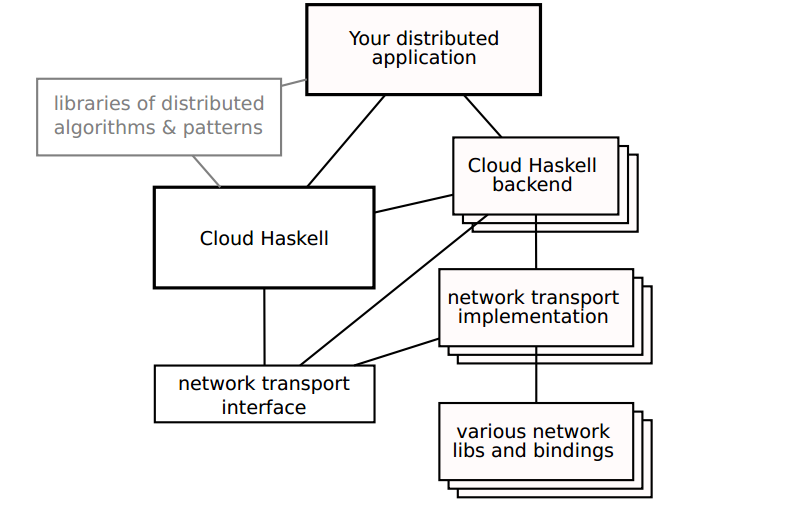
\includegraphics[width=\linewidth]{design}


\subsubsection{Serializing in absence of reflection!}
\label{sec:seri-absence-refl}

Haskell does not have reflection since the ability to inspect the
types at run-time would break referential transperancy. One of the
main contributions of Epstein et. al. \cite{epstein2011towards} was in supporting
serialization of function closures without reflection. Most of the
languages provide explicit support for serialisation in their run time
system. However, we don't want to add serialization machinery into the
runtime system for the following reasons :
\begin{itemize}
\item Loss of flexibity. We want to have explicit control over how to
  serialize types for performance and efficiency reasons. This is the
  advantage of using Type Classes in Haskell.
\item We want to enforce the constraint that some types are not
  serializable. Receive ports, MVars and TVars are example of type that
  should not be serialized. 
\item Explicitly serializing makes the cost model of sending it over
  the nework explicit and visible to the programmer.
\end{itemize}

The key insight was that the the closure of a function does not
depends on its type. Instead it depends on whether it has free
variables or not. Both serialization and deserialization are performed
as closure construction time not at closure-serialization time. For
more details refer to \cite{epstein2011towards}. 

\subsubsection{Typed Channels}
\label{sec:typed-channels}

The other unique feature that is not available in Erlang is the
abitlity to have multiple channels between 2 processes of different
types. So , we can get static guarantees about the types of values
that we are going to send/receive across a particular channel. The
usefulness of such a feature is currently unexplored. Furthur
experiments and implementations would illustrate whether this would be
very useful to the programmer.

\subsubsection{Shared Concurrency and STM support}
\label{sec:shar-conc-stm}

Unlike in Erlang which is a very primitive language without support
for Shared Memory Concurrency and Software Transactional Memory,
Haskell already has very good support of such features. Therefore
programmer has the flexibilty of using multiple concurrency models in
the same program. For example if processes are running on multi-core
processors, they can share threads and STMs can prove to be a useful
abstraction for managing concurrency within a node. This would be an
advantage in future when large scale distributed clusters would be of
hybrid nature with large number of cores on each nodes.

\subsubsection{Error Handling}
\label{sec:error-handling}

Errors are everywhere in distributed programming. The right thing to
do is to assume that processes will fail. A communication loss counts
as failure. In such a scenario , interested process should be
notified.

One major way in which Cloud Haskell differs from Erland is the way it
handles node disconnect and reconnect. Current Erlang implementation
does not gurantee reliability. Intermittent messages may be dropped if
the recieving node disconnects and reconnects. Although future
semantics of erlang talks about keeping the reliabilty property by
buffering messages to disconnected nodes, implementing it properly is
quite impossible. The cloud haskell semantics states that messages are
dropped permanently in case of a disconnected nodes. But it provides
an explicit reconnect primitive to accept intermediate message loss.
The process simply fails on initial disconnect. Any process that wants
to handle reconnect explicity has to opt in and accept the reality of
message loss.

%------------------------------------------------

\section{Apache Pig}
\label{sec:apache-pig}

Pig Latin is a scripting language which takes a sql like script as
input and produces MapReduce Java code which can be run on Hadoop cluster\cite{wiki_pig}

\subsection{Example}
\label{sec:example}

Here is an example of a program which computes the average pagerank of categories.

\begin{Verbatim}[frame=single]
  good_urls = FILTER urls BY pagerank > 0.2 groups = GROUP good_urls
  BY category big_groups = FILTER groups BY COUNT(good_urls) > 10^6
  output = FOREACH big_groups GENERATE category,
  AVG(good_urls.pagerank)
\end{Verbatim}

The above program will generate parallel executable tasks which can be
distributed across 1,000s of machines in a Hadoop cluster to count the
number of words in a dataset such as "all the webpages on the
internet".

\subsection{Impact}
\label{sec:impact}

Map Reduce is a low level programming environment for such queries.
Pig-Latin accepts high-level queries and converts them into a set of
map-reduce jobs.

A standard Pig-Latin script is 20x shorter than its equivalent java
code and takes the programmer 16x less time to implement. Moreover,
its only slightly slower than a hand written java program. Hence, it
is used quite frequently in the industry. At Yahoo!, currently about
90 percent of Hadoop jobs are written in PigLatin. It is also heavily
used by Twitter, AOL, Nokia, LinkedIn, etc.

\section{Pig In Cloud Haskell}
\label{sec:pig-cloud-haskell}

We propose a Pig like DSL on top of CloudHaskell which would do away
with lot of boilerplate code being written for distributed tasks.
Besides, Haskell is quite well-suited for writing DSLs. Generalised
Abstract Data Types (GADTs) would be useful for implementing such a
DSL.
The example shown below implements an Expression Evaluator in Haskell.

\begin{lstlisting}
data Expr =    I Int            -- integer constants
             | Add Expr Expr    -- add two expressions
             | Mul Expr Expr    -- multiply two expressions

eval :: Expr -> Int
   eval (I n)       = n
   eval (Add e1 e2) = eval e1 + eval e2
   eval (Mul e1 e2) = eval e1 * eval e2
\end{lstlisting}

Our proposed implementation would look like something similar 

\begin{lstlisting}
data Stmt =  Load Relation
             | Filter Relation
             | Group Relation By Category

data Relation 
  and so on ...   

\end{lstlisting}

Given a Map-Reduce Framwork on top of Cloud Haskell with well defined
semantics, we can convert Pig-Latin statements as composition of Map
Reduce functions.

\section{Conclusion}
\label{sec:conclusion}

The support for distributed programming in Haskell is very recent. The
basic toolkit is not there yet for writing Hadoop like jobs.
Nevertheless, the feature set seems promising and Haskell seems to be
at a very good position to tackle the problem of programming large
scale clusters. The most popular approach, MapReduce, pioneered by
Google, is infact a rudimentary primitve in functional programming.
Who knows what else higher order abstractions supported in Functional
programming in general and Haskell in particular would become
mainstream in Cloud Computing in the years to come!

%------------------------------------------------


\bibliographystyle{plain}	% (uses file "plain.bst")
\bibliography{refs}		% expects file "myrefs.bib"
%\end{multicols}
\end{document}
